\section{Introduction}

Due to the continual deployment of new applications and network technologies, and changes in workload patterns, research on congestion control has not only remained vibrant since the 1980s, but has flourished in recent years. Figure~\ref{fig:cctimeline} shows a time-line of innovations in this area.

At its core, a congestion control protocol determines when each segment of data must be sent. Because a natural place to make this decision is within the transport layer, congestion control today is tightly woven into kernel TCP software and runs independently on each TCP connection.

%However, this tight coupling is not fundamental to congestion control; rather,
%it imposes an artificial restriction on algorithms to restrict their
%computations to a single packet inter-arrival time lest they slow down the
%flow.
%Newly proposed algorithms lacking kernel implementations, such as
%PCC~\cite{pcc}, Nimbus~\cite{nimbus}, Remy~\cite{remy}, and
%Sprout~\cite{sprout}, all involve calculations that are cumbersome to perform in
%the kernel, and are challenging to engineeer to meet tight performance
%requirements.
%For example, Nimbus uses Fast Fourier Transforms to determine the amount and
%nature of the cross-traffic on the bottleneck link.

An operating system's TCP software is but one example of a {\em datapath}, the term we use for any module that provides data transmission and reception interfaces between higher-layer applications and lower-layer network hardware. Recently, many other datapaths have emerged, including user-space protocols atop UDP (e.g., QUIC~\cite{quic}, WebRTC~\cite{webrtc}, Mosh~\cite{mosh}), kernel-bypass methods (e.g., mTCP/DPDK~\cite{dpdk,mtcp,netmap}), RDMA~\cite{dcqcn}, multi-path TCP (MPTCP)~\cite{mptcp}, and specialized Network Interface Cards (``SmartNICs''~\cite{smartnic}). This trend suggests that the future will likely see many applications using datapaths different from kernel-supported TCP connections.

\begin{figure}[t]
\centering
    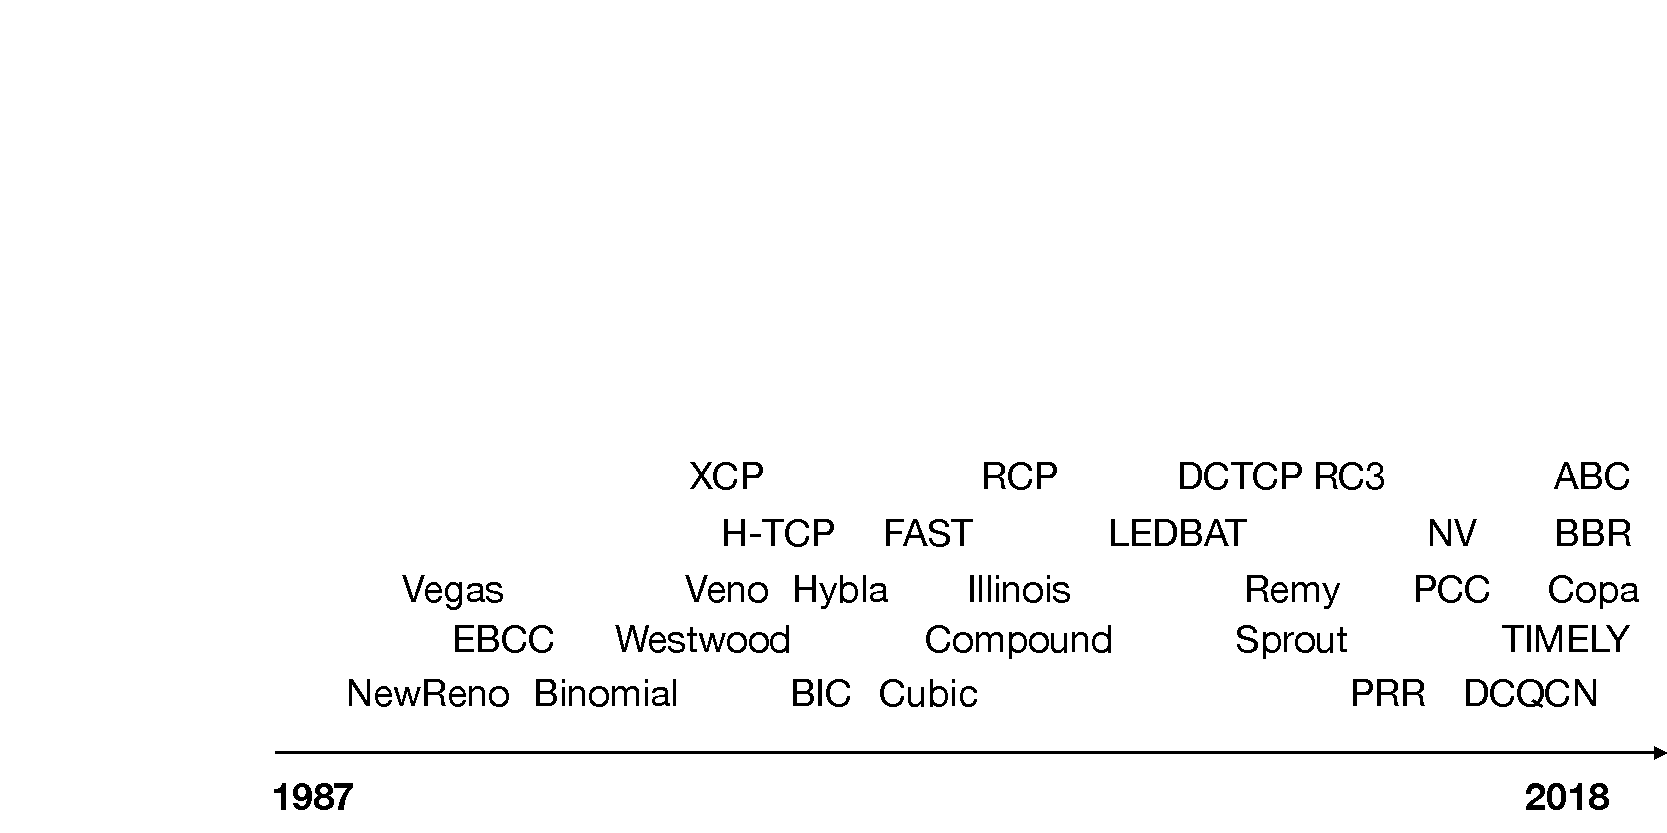
\includegraphics[width=\columnwidth]{img/cc-timeline-nocongsig}
    \vspace{-1cm}
    \caption{As link characteristics diversify, developers have developed a battery of congestion control algorithms, from the ``long-fat pipe'' schemes of the mid-2000s~\cite{westwood, veno, htcp, hybla} to purely delay-based~\cite{vegas, fasttcp, ledbat, nv, timely} and hybrid loss-delay~\cite{illinois, compound} schemes, and more recent proposals~\cite{pcc, remy, sprout, bbr, copa, abc}.}\label{fig:cctimeline}
\end{figure}

New datapaths typically do not offer much in terms of congestion control because implementing these algorithms correctly takes considerable time and effort. For instance, the set of available algorithms in mTCP~\cite{mtcp}, a TCP implementation on DPDK, is limited to a variant of Reno. 
Lest one dismiss this example as a case of a research project lacking in engineering resources, we note that QUIC, despite Google's imposing engineering resources, does not have most of the algorithms that have been implemented in the Linux kernel over many years.  
We expect this situation to worsen with the emergence of new hardware accelerators and programmable network interface cards (NICs) because high-speed hardware designers tend to forego programming convenience for performance. The difficulty isn't the volume of code, but the many subtle correctness and performance issues in various algorithms that require expertise to understand and resolve.

This paper starts from the observation, made in a recent position paper~\cite{ccp-hotnets}, that congestion control algorithms do not need to be implemented in the datapath. If the datapath encapsulated the information available to it about {\em congestion signals} like the round-trip time (RTT), packets received and lost, explicit congestion notification (ECN) markings, etc., and periodically provided this information via a well-defined interface to an off-datapath module, then congestion control algorithms could run in the context of that module. Then, by exposing an analogous interface to control transmission parameters such as the window size, pacing rate, and transmission pattern, the datapath could transmit data according to the policies of the off-datapath congestion control algorithm. 
Of course, the datapath (\eg Linux kernel TCP stack) must be modified to expose
such an interface, but such an effort only needs to be undertaken once for each
datapath, and does not grow with the number of congestion control algorithms.

We use the term {\em Congestion Control Plane (CCP)} to refer to this off-datapath module. Running congestion control in the CCP offers the following benefits:
\begin{enumerate}
    \item {\bf Write-once, run-anywhere:} With CCP, one can write a congestion control algorithm once and run it on any datapath that supports the specified interface. 
    We demonstrate in this paper a variety of algorithms running on three datapaths: the Linux kernel, mTCP/DPDK, and QUIC, and show algorithms running for the first time on certain datapaths (e.g., Cubic on mTCP/DPDK, Copa on QUIC).
    \item {\bf Higher ``velocity'' of development:} With the right abstractions,
      a congestion control designer can focus on the algorithmic essentials
      without worrying about the details and data structures of the
      datapath. 
    The result is more expressive, easier to maintain code. We
      enable a deployment mode where CCP and the algorithm run at user level,
      implemented in Rust or using CCP's Python bindings. 
    If the kernel module implementing CCP support is upstreamed, any new algorithms
      (including untrusted ones) can be deployed into high performance
      production systems over Linux without involving the upstreaming process.

    \item {\bf New capabilities:} CCP makes it easier to provide new
      capabilities, such as aggregate control of multiple flows as previously
      proposed in the congestion manager~\cite{cm}, and freedom from the ``ACK
      Clock'' for algorithms that require significant computation (e.g., signal
      processing, machine learning, \etc). 
    All the benefits of a \userspace
      programming environment (libraries, debuggers, \etc) will be available to
      developers.
\end{enumerate}

\vspace{0.1in}
In summary, this paper contributes:

\begin{itemize}
\item A high-level event-driven language to specify congestion control
  algorithms. Algorithm developers specify congestion control behavior using
  combinations of events and conditions, such as the receipt of an
  acknowledgment or a loss event, along with corresponding handlers to perform
  simple computations directly in the datapath (\eg increment a window) or defer
  complex logic to a userspace component.

\item A specification of datapath responsibilities. These include congestion
  signals that a datapath should maintain (Table~\ref{tab:api}), as
  well as a simple framework to execute directives from a CCP program. This
  design enables ``write-once, run-anywhere'' protocols.

\item A preliminary demonstration of new capabilities enabled by CCP, including
  sophisticated new congestion control algorithms and the implementation of an
  aggregate congestion controller acting on behalf of multiple flows.

\item An evaluation of the fidelity of CCP relative to in-kernel
  implementations under a variety of link conditions. Our CCP implementation
  matches the performance of Linux kernel implementations at only a small
  overhead (5\% more CPU utilization in the worst case).
  Furthermore, we show it
  is feasible to implement infrequent congestion control even in low-RTT, high
  bandwidth environments.

\end{itemize}
